\documentclass{acm_proc_article-sp}
\usepackage[utf8]{inputenc}

\renewcommand{\paragraph}[1]{\vskip 6pt\noindent\textbf{#1 }}
\usepackage{hyperref}
\usepackage{graphicx}
\usepackage{url}

\providecommand{\tightlist}{%
  \setlength{\itemsep}{0pt}\setlength{\parskip}{0pt}}

\title{Understanding Airbnb listings in Australia}


% Add imagehandling
\usepackage{graphicx}
% Redefine \includegraphics so that, unless explicit options are
% given, the image width will not exceed the width of the page.
% Images get their normal width if they fit onto the page, but
% are scaled down if they would overflow the margins.
\makeatletter
\def\ScaleIfNeeded{%
  \ifdim\Gin@nat@width>\linewidth
    \linewidth
  \else
    \Gin@nat@width
  \fi
}
\makeatother
\let\Oldincludegraphics\includegraphics
{%
 \catcode`\@=11\relax%
 \gdef\includegraphics{\@ifnextchar[{\Oldincludegraphics}{\Oldincludegraphics[width=\ScaleIfNeeded]}}%
}%

\numberofauthors{2}
\author{
\alignauthor Louelle Teo Fengmin \\
        \affaddr{Singapore Management University}\\
       \email{\href{mailto:louelle.teo.2020@mitb.smu.edu.sg}{\nolinkurl{louelle.teo.2020@mitb.smu.edu.sg}}}
\and \alignauthor Jason Tey Shou Heng \\
        \affaddr{Singapore Management University}\\
       \email{\href{mailto:jason.tey.2020@mitb.smu.edu.sg}{\nolinkurl{jason.tey.2020@mitb.smu.edu.sg}}}
\and \alignauthor Wong Kian Hoong \\
        \affaddr{Singapore Management University}\\
       \email{\href{mailto:kh.wong.2020@mitb.smu.edu.sg}{\nolinkurl{kh.wong.2020@mitb.smu.edu.sg}}}
\and }

\date{}

%Remove copyright shit
\permission{}
\conferenceinfo{} {}
\CopyrightYear{}
\crdata{}

% Pandoc syntax highlighting

% Pandoc citation processing
\newlength{\csllabelwidth}
\setlength{\csllabelwidth}{3em}
\newlength{\cslhangindent}
\setlength{\cslhangindent}{1.5em}
% for Pandoc 2.8 to 2.10.1
\newenvironment{cslreferences}%
  {}%
  {\par}
% For Pandoc 2.11+
\newenvironment{CSLReferences}[3] % #1 hanging-ident, #2 entry spacing
 {% don't indent paragraphs
  \setlength{\parindent}{0pt}
  % turn on hanging indent if param 1 is 1
  \ifodd #1 \everypar{\setlength{\hangindent}{\cslhangindent}}\ignorespaces\fi
  % set entry spacing
  \ifnum #2 > 0
  \setlength{\parskip}{#2\baselineskip}
  \fi
 }%
 {}
\usepackage{calc} % for calculating minipage widths
\newcommand{\CSLBlock}[1]{#1\hfill\break}
\newcommand{\CSLLeftMargin}[1]{\parbox[t]{\csllabelwidth}{#1}}
\newcommand{\CSLRightInline}[1]{\parbox[t]{\linewidth - \csllabelwidth}{#1}}
\newcommand{\CSLIndent}[1]{\hspace{\cslhangindent}#1}


\begin{document}
\maketitle

\begin{abstract}
\emph{(abstract of not more than 300 words)}

The abundance of Airbnb data provides great opportunity to conduct a
variety of data analyses to understand the residential short-lease
rental market. Most publicly available analysis tools of Airbnb data do
not have much interactive features and are therefore, by design, narrow
in their application and scope. This Shiny application provides an
analytics platform for interested parties such as analysts, especially
those who are not familiar with coding and programming languages, to
conduct exploratory spatial data analysis, text and sentiment analysis,
cluster analysis, and predictive analysis on the Australia Airbnb
dataset. No prior programming knowledge is required to use this
interactive dashboard, while the environment allows users to customise
their scope of analysis. This paper details the design framework, data
preparation and use case demonstration using the simple and
user-friendly interactive dashboards.
\end{abstract}

\hypertarget{introduction}{%
\section{Introduction}\label{introduction}}

\emph{{[}The actual research paper itself should not more than 6 pages
excluding figures, tables, formula and references.{]}}

Airbnb is an online marketplace platform for accommodation rental.
Founded in 2008 by Brian Chesky and Joe Gebbia who had the idea to put
an air mattress in their living room and offered bed \& breakfast{[}3{]}
(thus ``Airbnb''), the company has grown to be one of the most popular
short-term accommodation rental platforms in multiple countries around
the world.

With millions of listings in 220 countries and over 100,000
cities{[}1{]}, Airbnb has a rich store of data from transactions between
hosts and guests. Such data includes structured data like price, number
of facilities (e.g.~bedrooms, bathrooms), minimum and maximum number of
nights' stay; and unstructured text data such as description of the
accommodation, and reviews by guests. This paper utilizes such data
scraped by Inside
Airbnb{[}\textbf{http://insideairbnb.com/get-the-data.html?}{]} via the
Airbnb website to create an interactive dashboard that allows analyst or
anyone interested in the AirBnb landscape to conduct the statistical
analyses without the need of any prior coding or programming knowledge.
Analytic tools included in this dashboard are Exploratory Data Analysis;
Cluster Analysis; Exploratory Spatial Analysis; Text and Sentimental
Analysis; and Predictive Analysis.

\hypertarget{motivation}{%
\section{Motivation}\label{motivation}}

\emph{(Motivation of the application)}

AirBnb is one of the pioneers, larger player, and rapidly-growing
company in the increasingly important sharing economy of the world,
Given rich multitude of data made available through its website, there
are huge potential for a free-to-use analytical dashboard that housing
market analyst, sharing economy professionals, property agents, research
institutes, and would-be AirBnB hosts to utilise and better understand
this business environment.

However, analysts, hosts, and professionals who are keen to delve into
such data sets might not have the requisite knowledge or programmatic
skills to develop their own analytic tools. This application aims to
bridge this gap by providing a publicly available analytic dashboard
that provides various analytical techniques to enable interested parties
to tap on the rich data provided to derive meaningful insights for their
professional use. The target users of this application are analysts with
some knowledge of statistical techniques but lack the coding skills to
develop their own tools.

While this application focuses on the Australia Airbnb listings dataset,
the data processing, methodologies, and app development process can be
easily replicated and reproduced with datasets of other geographical
areas that bear the same data structure.

\hypertarget{review-of-past-works}{%
\section{Review of past works}\label{review-of-past-works}}

\emph{(Review and critique on past works)} There are currently a number
of analyses that has been conducted on the Airbnb dataset.

One of most prominent and recent study on Airbnb data is by Steve Deane
from Stratos, who wrote a blogpost in January 2021 on the topic. In his
post, Deane provides descriptive statistics. While some of the
statistics were provided, Deane's analysis is heavily weighted towards
the economic aspects of Airbnb. Deane does not provide any higher level
data analysis beyond the descriptive ones, with limited statistical
content and lacking in elaboration on how factors used were derived. The
major `flaw,' though, remains the fact that Deane's blog post is heavy
on qualitative write-up with minimal visualization - much less
interaactivity - of the statistics he quoted.

Several blog posts on provided basic guides on data analysis on the
Airbnb dataset. Kwon et. al.~(2018), Chen (2019), and Gedik (2020) are
some recent examples.

Kwon et. al.~(2018) used the Inside Airbnb listing data to apply Linear
Discriminant Analysis, Outliers were detected and removed using the
Cook's distance before a Box-Cox transformation was conducted to
normalize the data, and the dependent variable (review score) binned to
wrangle into categorical data type. Backward Elimination, Ordinal
Logistic Regression, and LASSO Regression methods were employed to
conduct explanatory analysis. The study concluded that number of
listings by hosts and having more bathrooms are crucial in securing
higher review score. While the study provided a well-rounded discussion
on the statistical methodoly, it does not offer interactive features to
allow other forms of data exploration or parameter adjustments.

Chen (2019) on the other hand provides an analysis that emphasized on
the geographical distribution of listings, and provided more data
visualizations that allow viewers to observe quick noticeable trends.
However, Chen was limited with her visualization choice (e.g.~showing
Average Price by Locations with equal-length bar differentiated by
colors on a continuous scale), and similarly does not provide
interactivity to conduct analysis that cater to needs of individual
analysts.

Comparatively, Gedik (2020) did a fairer job in terms of data analysis,.
However, similar to earlier studies, there is also no interactivity
offered to allow viewers autonomy in changing parameters.

Amongst all, Gupta (2019) provided the most well-rounded discussion and
presentation using the Airbnb listing data. Gupta aimed to provide an
exploratory analysis of Airbnb's data to understand the rental landscape
in New York City. He first employed descriptive time-series statistics
to map out the increasing trends in number of listings and reviews in
the city, before moving on to present an interactive Shiny App that
provides information on individual listing based on sets of filters
(e.g.~max budget, number of people, minimum rating). While Gupta offered
some form of interactivity, the Shiny does not provide any meaningful
insights, and is essentially a replica of the user interface offered by
Airbnb via the official website.

Within the industry, there exists interactive tools that allow analysts
and potential hosts to analyze rental data using attributes and past
performance. One such example is AIRDNA. Notwithstanding the fact that
the platform only offers paid services, the results are also provided in
a prescriptive manner with little analytical value-add, and limited
customisation for users to tweak the analysis to their individual
requirements.

\hypertarget{design-framework}{%
\section{Design Framework}\label{design-framework}}

\emph{(A detail description of the design principles used and data
visualisation elements built (Refer to Section IV: Interface of
\href{https://ink.library.smu.edu.sg/cgi/viewcontent.cgi?article=2760\&context=sis_research}{this
paper}.)}

The application makes use of the R stastical language which is
open-source and offers many tried-and-tested packages for the type of
analysis that the application will feature. The design considerations
are as follows:

\begin{enumerate}
\def\labelenumi{\arabic{enumi}.}
\tightlist
\item
  Reproducibility of results by performing calculations within the
  application itself.\\
\item
  Adoption of common R packages in the Comprehensive R Archive
  Network{[}8{]} (CRAN) for supportability.\\
\item
  Use of the R Shiny package for interactivity and easy deployment.\\
\item
  Offer interactive features for easy use.
\end{enumerate}

\hypertarget{data-preparation}{%
\subsection{Data Preparation}\label{data-preparation}}

All data preparation was performing using R in the RStudio IDE. This
included dropping columns from the data set that were irrelevant for the
scope of our research, converting columns into the appropriate data
types, and imputing NA values where appropriate.

\hypertarget{exploratory-data-analysis}{%
\subsection{Exploratory Data Analysis}\label{exploratory-data-analysis}}

\emph{(Can refer to Raymond Teo's paper:
\url{https://wiki.smu.edu.sg/1920t2isss608/Group11_research_paper} and
how they write this portion.)}

Exploratory Data Analysis (EDA) is an approach to data sets to summarise
their main characteristics. With EDA, we can - Propose hypotheses to
explain the observed characteristics of the data - Assess the data sets
and observe any anomalies and outliers - Support the selection of
appropriate statistical tools and techniques - Provide a basis for
further data collection through surveys and experiments

\hypertarget{barcharts}{%
\subsubsection{Barcharts}\label{barcharts}}

Barcharts in our Shiny will showcase the number of Airbnb listings or
hosts per \emph{State} and \emph{Local Government Area} (LGA). This
allows users to understand their market share and competition in the
area they are in. It also allows analyst to understand the different
states and tourism density.

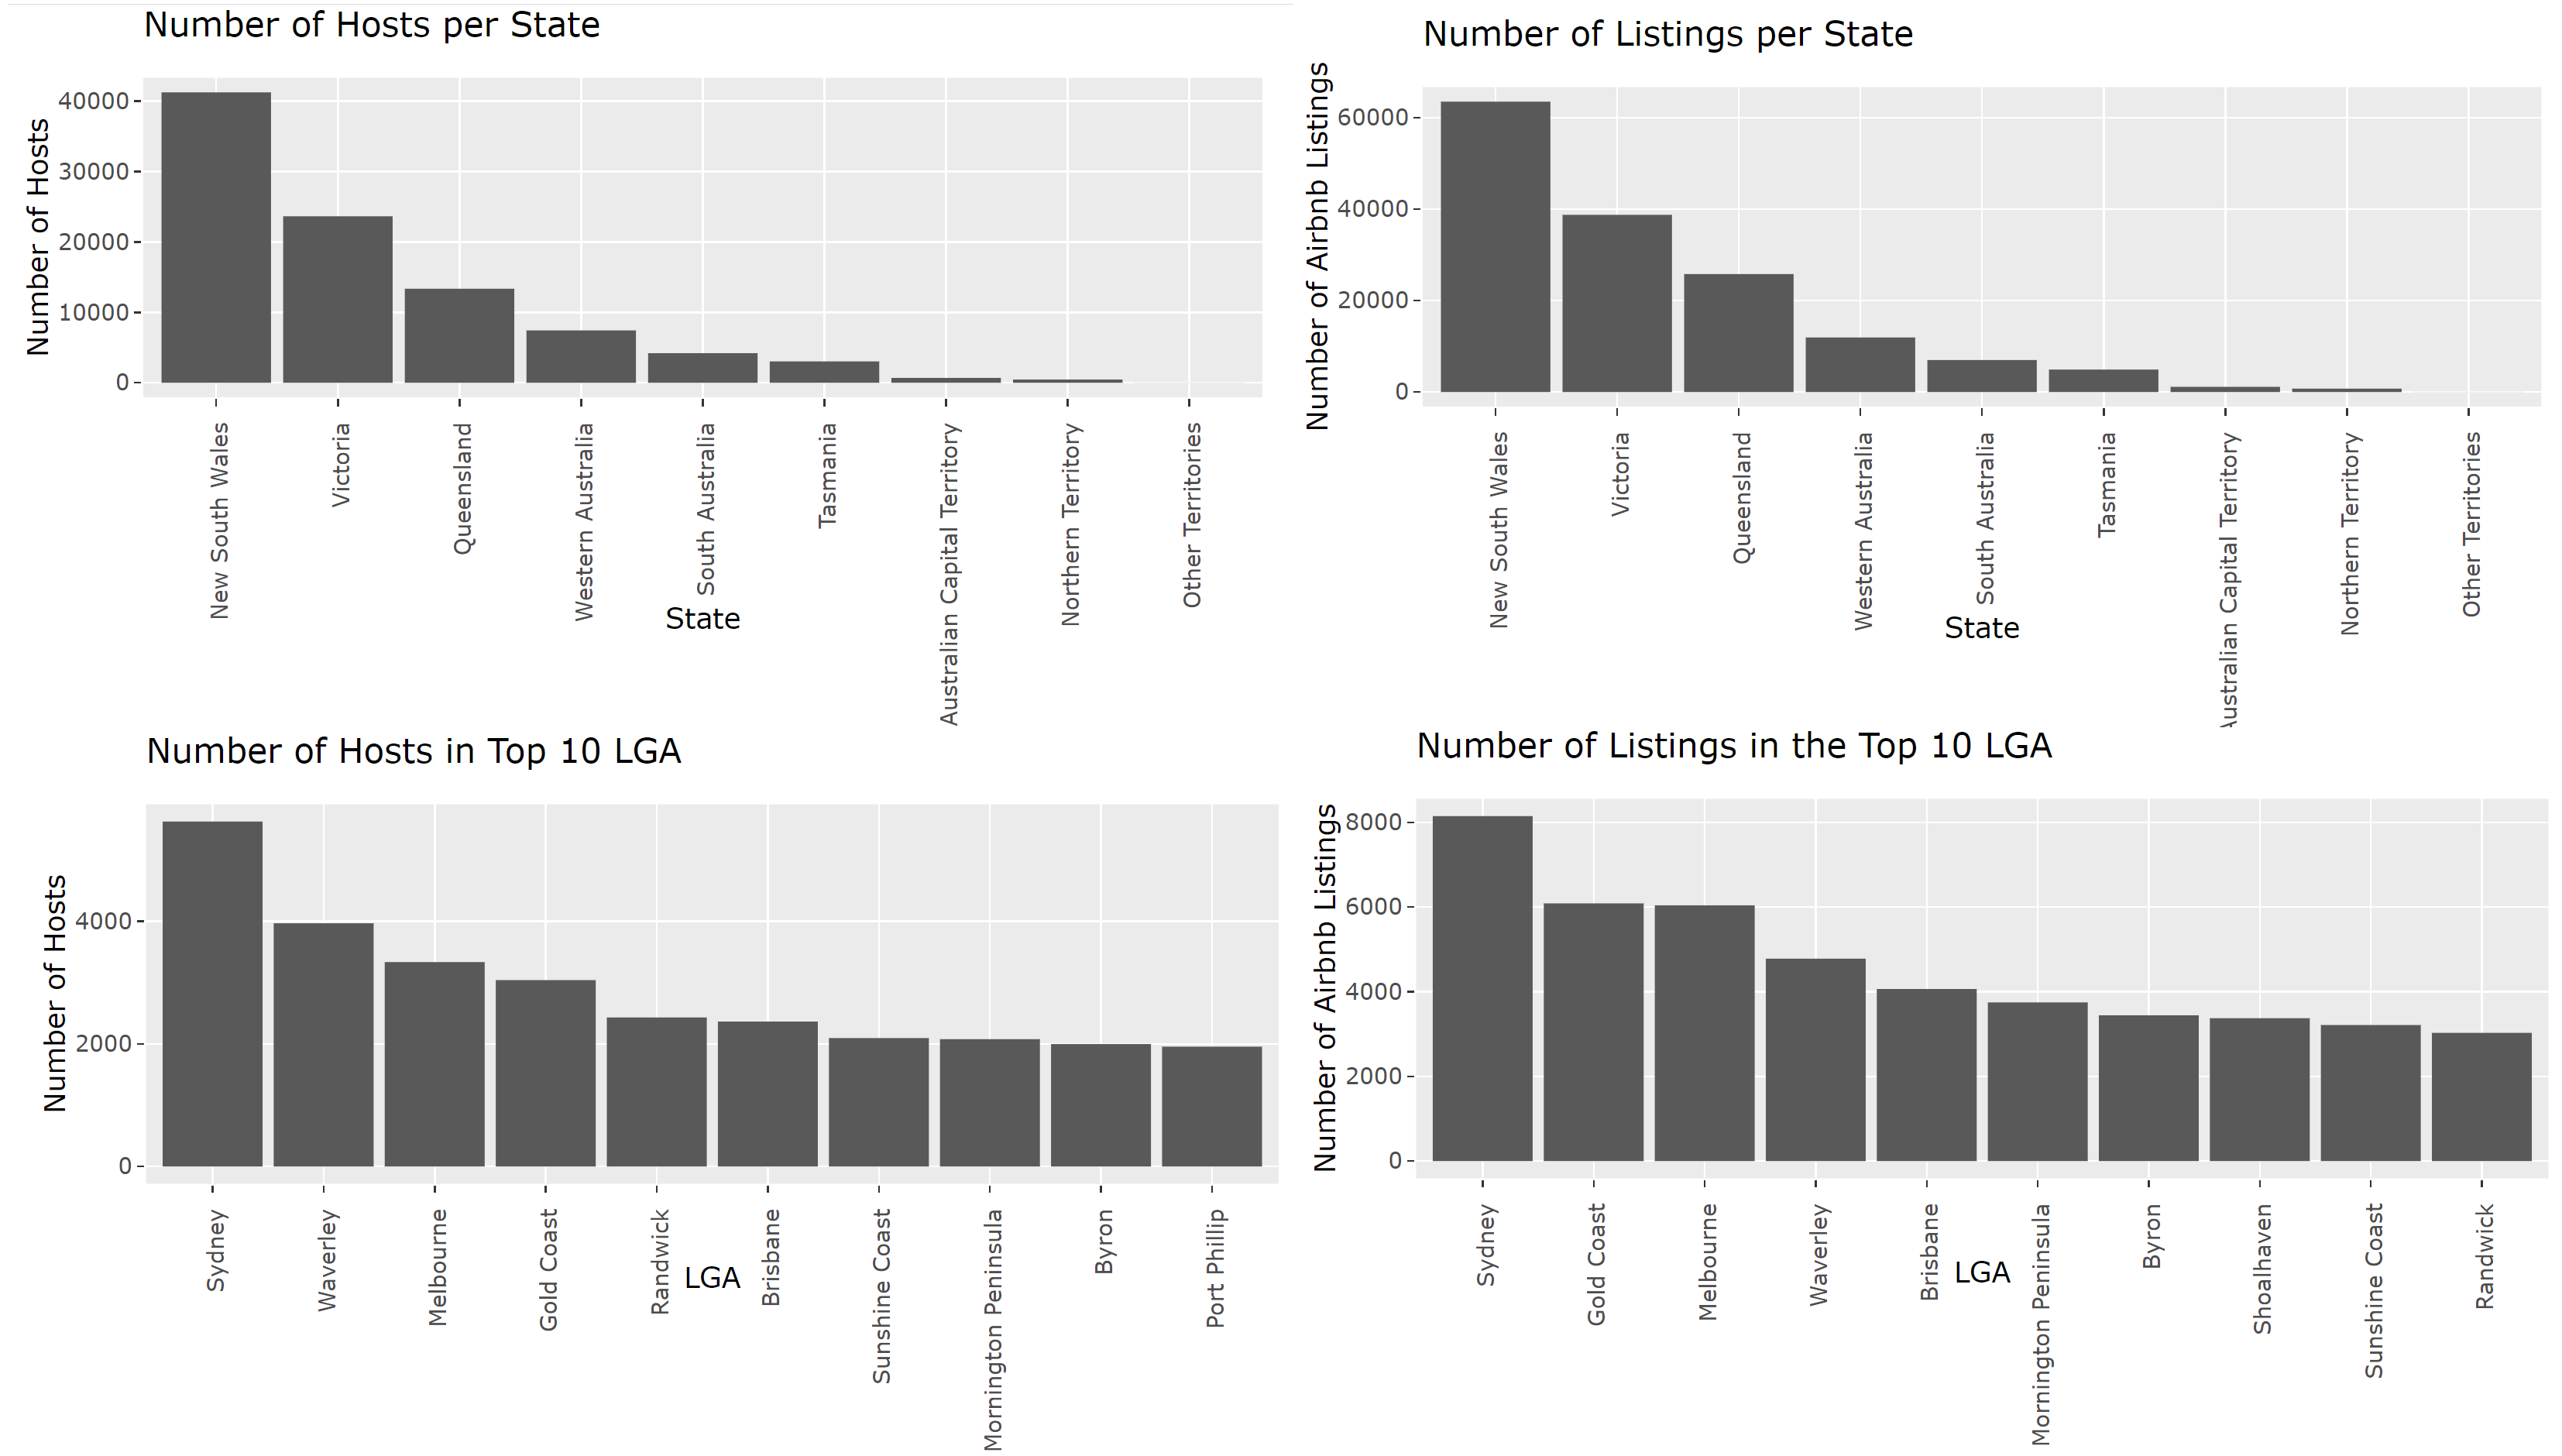
\includegraphics{images/hostlistings.png}

\hypertarget{boxplots}{%
\subsection{Boxplots}\label{boxplots}}

Boxplots in the shiny allows us to explore statistical data of the
different variables in each LGA, or per \emph{Property Type}. It is a
convenient way of depicting groups of numerical data through their
5-number summaries. - Smallest Observation - Lower Quartile - Median -
Upper Quartile - Largest Deviation

In this shiny, users will be able to toggle between different numerical
data to analyse the boxplots in different LGA.

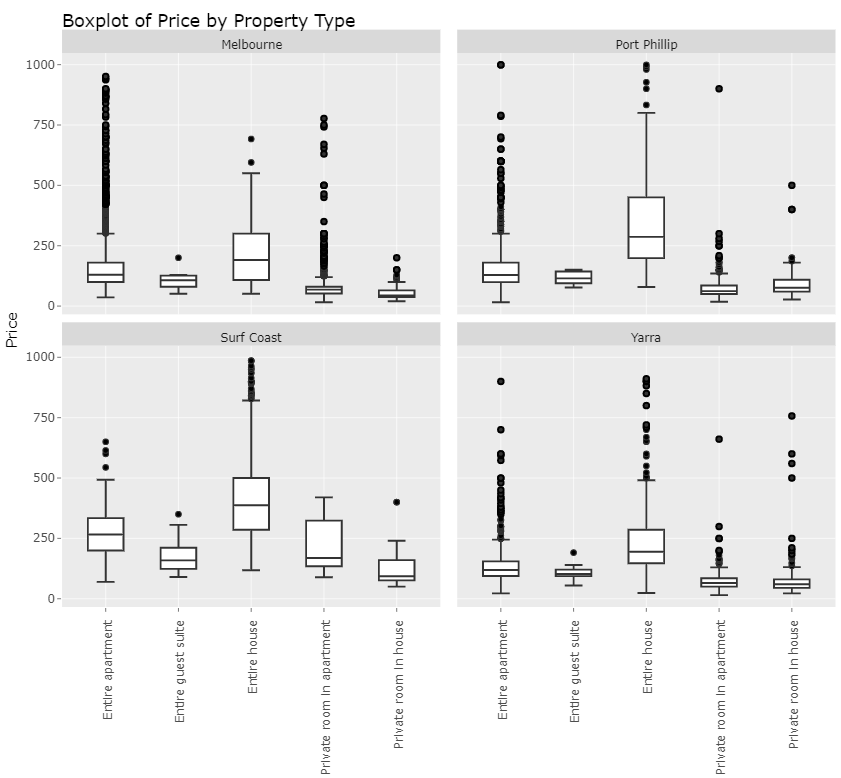
\includegraphics{images/boxplotvic.png}

\hypertarget{density-bivariate-analysis}{%
\subsection{Density \& Bivariate
Analysis}\label{density-bivariate-analysis}}

The Density plot allows users to understand where most of the data is
populated within the range. Therefore they are able to zoom in at the
denser clusters to do a better analysis.

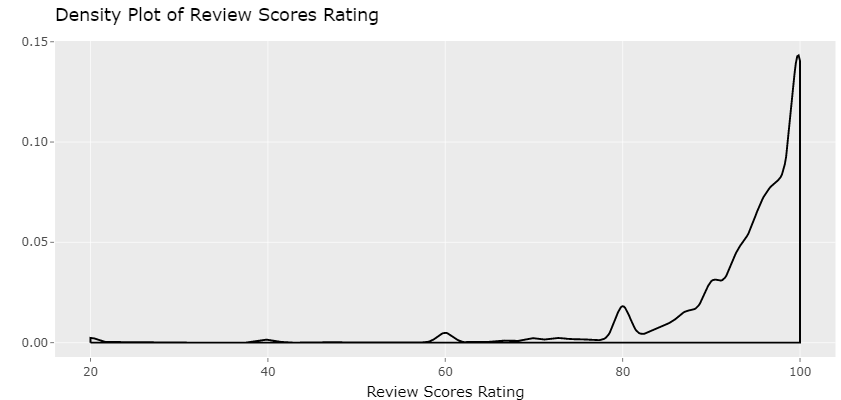
\includegraphics{images/densityplot.png}

The bivariate plot we will be using for this report is for two
continuous data. It allows us to consider the relationship between 2
variables.

For example, for below, we can see that there is a small positive linear
relationship between \emph{Review Scores Rating} and \emph{Price}.

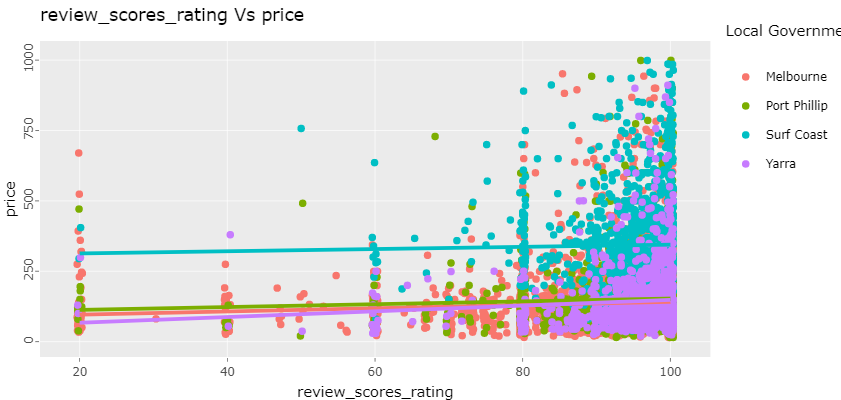
\includegraphics{images/bivariate.png}

\hypertarget{correlation-plot}{%
\subsubsection{Correlation Plot}\label{correlation-plot}}

\hypertarget{cluster-analysis}{%
\subsection{Cluster Analysis}\label{cluster-analysis}}

\emph{(Can refer to Raymond Teo's paper:
\url{https://wiki.smu.edu.sg/1920t2isss608/Group11_research_paper} and
how they write this portion.)}

\hypertarget{spatial-data-analysis}{%
\subsection{Spatial Data Analysis}\label{spatial-data-analysis}}

The spatial data analysis provides an analytical overview of the
geographical distribution of different variables of interest across the
different Local Government Areas (LGAs) of Australia. For example, the
choropleth below presents the median price of listing is in each of the
LGAs in the Victoria State - the darker the color, the higher the median
price for that LGA, and we see the darkest range of median price in the
area around the tip of the Melbourne bay. This way, we can easily
compare whether median prices are within the same range, higher, or
lower across the different LGAs.

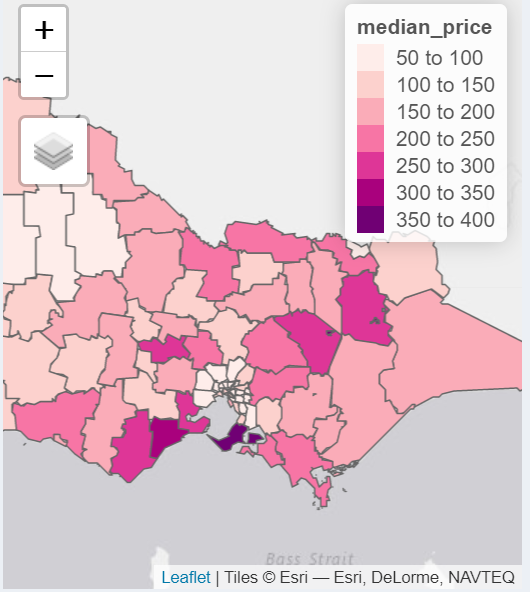
\includegraphics{images/geo1.png}

The above visualization is achieved by merging the Airbnb listings data
scrapped by Inside Airbnb (including the coordinates of each listing's
geospatial position) with the LGA digital boundaries in ESRI Shaprefile
format made available by the Australian Bureau of Statistics{[}2{]}.
Firstly, six variables from the raw listing data (i.e.. price, count,
ratings, number of reviews, acceptance and response rates) are
summarized and grouped using the base R \emph{summarise()} and
\emph{group\_by()} modules into their LGAs to obtain aggregated
variables.

Next, we import the shapefile using the \emph{st\_read} function from
the \emph{sf} package. We then left-join the summarized aggregated
values onto the spatial dataframe.

Finally, we remove rows that have missing values from our data, filter
data down to the state we are interested in (Victoria in this case) and
then plot the viz using functions under the \emph{tmap} package.\\
Beyond the selection of state, the application also allows user to tweak
the parameters, such as the variable of interest (6 in total) and
binning methods.

However, we also observed that there are LGAs of lower median price
north of the bay Melbourne Bay area) and clusters of higher median
prices (south-west of the bay). While good for overall distribution, the
choropleth does not provide an objective view of how the variable
(e.g.~median price) of one LGA compares with the other LGAs around ir or
across Australia. We hence aim to identify clusters based on variable of
interest to identify ``hot/cold spots'' and outlier LGAs. To do this, we
employ a Local Indicators for Spatial Autocorrelation (LISA) analysis,
which helps to reveal clusters of LGAs/outliers based on their
attributes.

The first step to determining the local spatial autocorrelation is to
determine what constitutes a neigboring area to consider and hence the
spatial weight to be assigned for analyzing association. There are
several ways to do this, categorized mainly into two types: (i)
contiguity-based{[}6{]} and (ii) distance-based{[}7{]}. (i) is further
split into Queen's contiguity (with shared vertex - no shared border
needed) and Rook's contiguity (smaller distance threshold; only shared
borders), analogous to a chess board; (ii) is also further split into
K's Nearest Neighbor (i.e.~the K LGAs nearest to subject,
centroid-to-centroid) and Distance-band (any area with centroid within a
distance band radius from subject centroid). The neighbor spatial
weights are derive using the respective modules within the \emph{spdep}
package.

The resultant spatial weight and spatial dataframe is then used to
derive the LISA - in this case, the Local Moran's I (note: Getis-Ord's G
Z-score is also available; discussion and application is available via
\href{https://onlinelibrary.wiley.com/doi/pdf/10.1111/j.1538-4632.1992.tb00261.x}{this}
and
\href{http://personal.tcu.edu/kylewalker/spatial-neighbors-in-r.html}{this
link} respectively; the latter was used as a reference to develop this
sub-module). We then use the \emph{localmoran} function from the same
\emph{spdep} package to calculate the Local Moran's I statistics for
each of the LGAs. The underlying formula is given as follows:

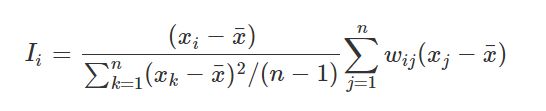
\includegraphics{images/lmformula.png}

where x(i) is the variable of interest for LGA i, w(ij) the spatial
weight with neighbor j, and x-bar the mean. The statistic is then tested
for statistical significance - LGAs with statistically significant
statistic rejects null hypothesis that they are no spatial associated
with their neighbors - these LGAs are then further categorized into four
classes based on their deviation from the mean. If an LGA's variable of
interest is higher than its mean, it has a comparatively high value; if
its local Moran's is higher than the statistic's mean, the neighbors
also have high values - this thus presents a High-High cluster. A
summary of the four clusters is presented below:

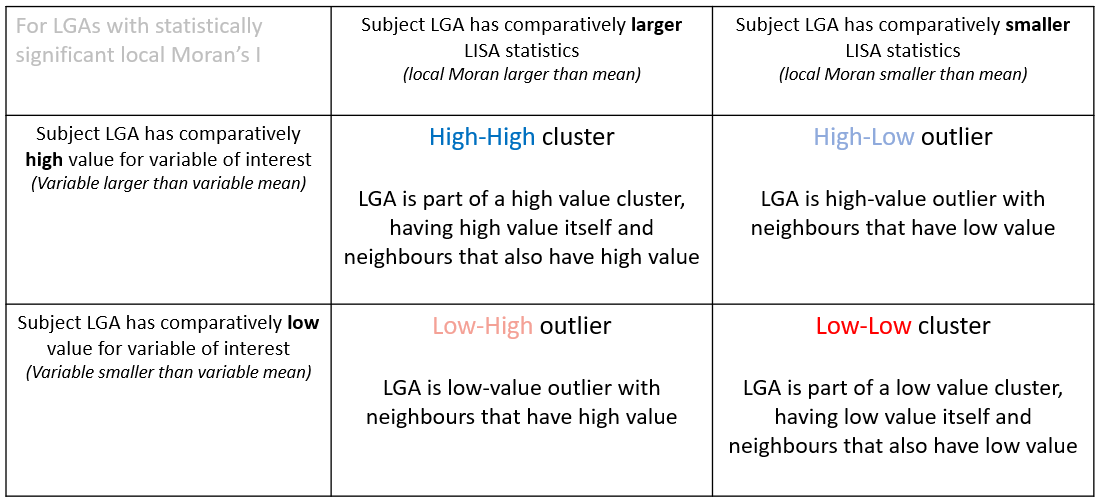
\includegraphics{images/lminterpret.png}

The resultant LISA analysis for median price in LGAs in the State of
Victoria is as shown below. The areas shaded (regardless of which
cluster/outlier the LGA belongs to) on the right-hand viz according to
the confidence level selected (90\%, the default, in the viz below)
should correspond to the p-value of the left-hand viz (all the colored
area has p-value corresponding to 90\% confidence level and above). The
methods of selecting neighbor and the confidence level for the
statistical analysis can be varied according to user preference.

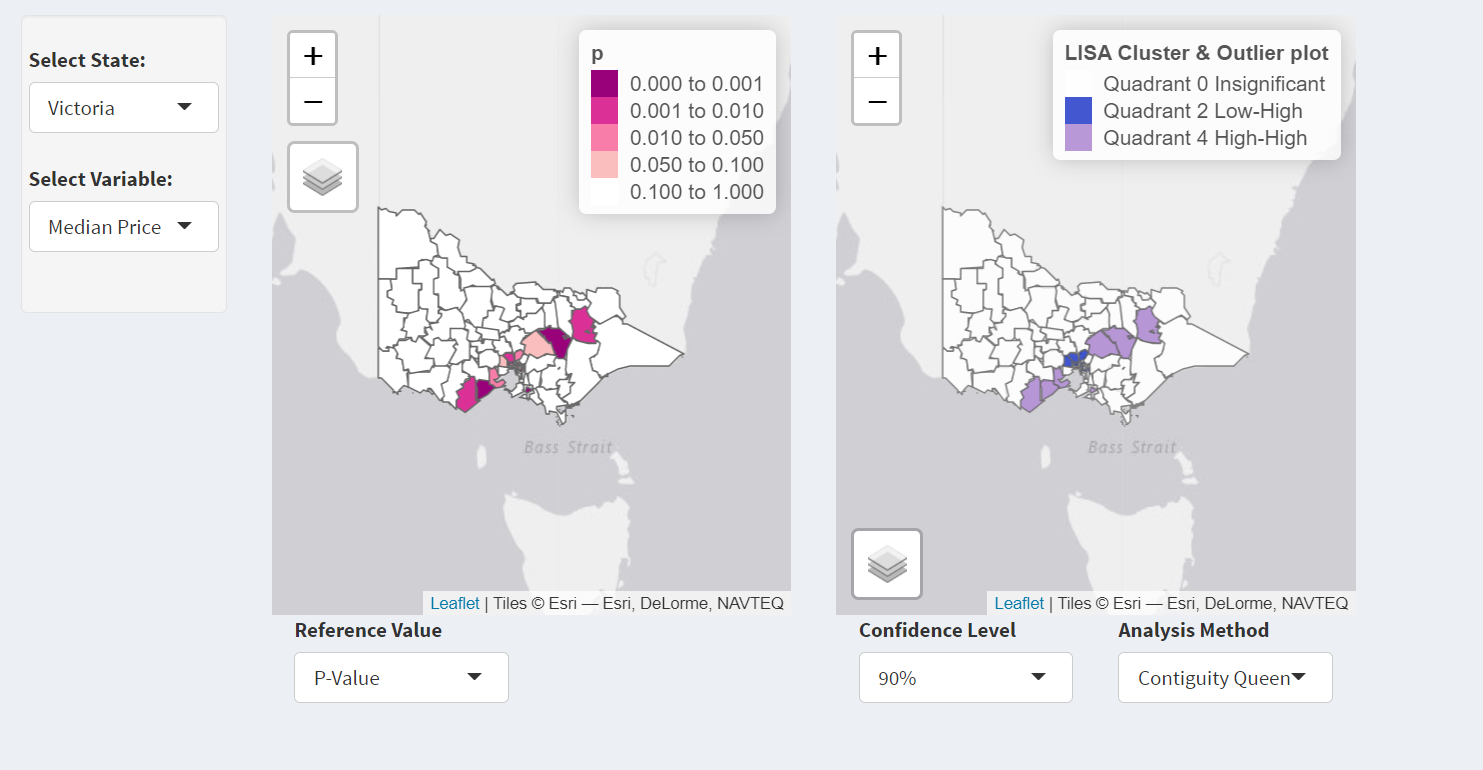
\includegraphics{images/geo2.png}

\hypertarget{sentiment-analysis}{%
\subsection{Sentiment Analysis}\label{sentiment-analysis}}

\emph{(Can refer to Raymond Teo's paper:
\url{https://wiki.smu.edu.sg/1920t2isss608/Group11_research_paper} and
how they write this portion.)}

\hypertarget{word-cloud}{%
\subsubsection{Word Cloud}\label{word-cloud}}

Word clouds are an effective way to represent the frequency that a word
appears in a particular corpus (a collection of texts). For this
application, the size of the word represents the relative frequency of
the word in the description section of Airbnb listings. The word in the
largest font is the most common word.

The first step to clustering is to create the corpus. This is done by
scraping all the text from the desired column in the Airbnb data set -
in this case, the description field. Once the corpus is created,
tokenisation is done to clean up the words or terms and create a tibble
of single terms in a column. Tokenisation includes removing extra white
spaces from between terms, removing numbers (number do not have any
meaning in a textual word cloud), punctuation symbols, and removing
\emph{stop words} (which refer to words that have no meaning like ``I,''
``a,'' ``this,'' ``and,'' etc), and stemming words (reducing words to
their root like ``walking'' to ``walk''). This cleaning process ensures
that only valuable terms are included.

After tokenisation is performed, the corpus of words are transformed
into a Document Term Matrix (DTM), which is a matrix of the frequency of
each term in the corpus. Based on the DTM, the word cloud will generate
the words according to their frequency.

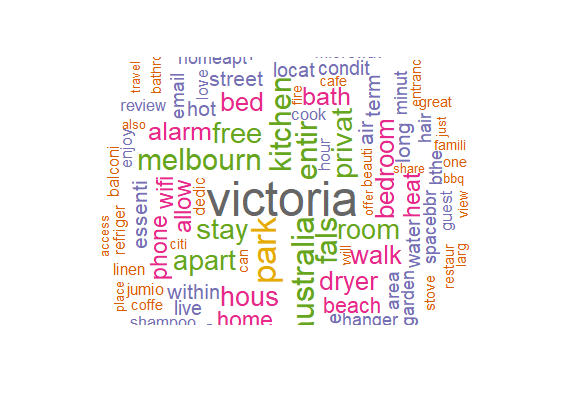
\includegraphics{images/wordcloud1.png} \emph{Figure 1: Word Cloud}

\hypertarget{topic-modelling-using-latent-dirichlet-allocation}{%
\subsubsection{Topic modelling using Latent Dirichlet
Allocation}\label{topic-modelling-using-latent-dirichlet-allocation}}

Topic modelling is a statisical model to identify topics in textual
data. It is an unsupervised machine learning technique that detects word
and phrase patterns in documents and clusters them into groups known as
topics. The concept behind topic modelling is that different topics
would have certain words appear together frequently. Based on this,
topics can be discovered based on the words that appear frequently
together.

The 2 common approaches to topic modelling are Latent Semantic Analysis
(LSA) and Latent Dirichlet Allocation (LDA){[}4{]}.

As described by Cvitanic, et al. {[}4{]}, LSA is a text analysis method
that makes use of a semantic space (representations of natural language
meant to identify meaning in language) to calculate or compute the
similarity between words, phrases, sentences, paragraphs, or even whole
documents. Similar to the word cloud, LSA makes use of a document term
matrix to weight the words in terms of the frequency that they appear in
the corpus.

LDA, according to Cvitanic, et al. {[}4{]} was a topic modelling
technique that evolved from LSA. The basic idea of LDA is that
``documents are represented as random mixtures over latent topics, where
each topic is characterized by a distribution over words.''{[}4{]} To be
able to identify the topics in a corpus, a ``generative process whereby
the documents are created'' is done so as to infer the topics{[}5{]}.
This inference is done by imagining documents being random mixtures of
terms with latent topics underlying them, where each topic has a unique
distribution across all the words in the corpus{[}5{]}. LDA requires a
defined number of topics as an input parameter.

In other words, LDA assumes that all words in the document can be
assigned a probability of belonging to a topic. As such, the goal of LDA
is to determine the mixture of topics that a document contains.

LDA was chosen at the topic modelling technique to implement in this
application.

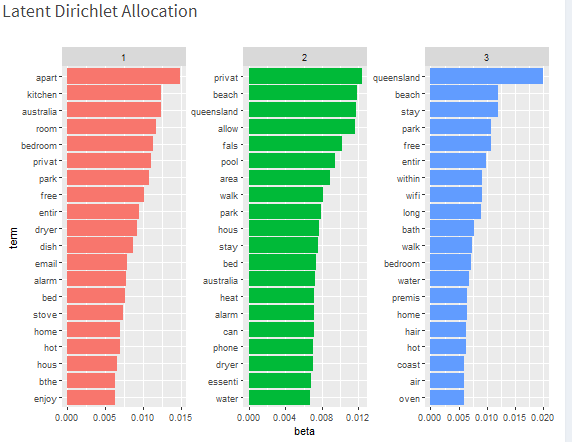
\includegraphics{images/topicmodel1.png} \emph{Figure 2: Topic Modelling
using LDA}

\hypertarget{multi-linear-regression-analysis}{%
\subsection{Multi-linear Regression
Analysis}\label{multi-linear-regression-analysis}}

\emph{(Can refer to Raymond Teo's paper:
\url{https://wiki.smu.edu.sg/1920t2isss608/Group11_research_paper} and
how they write this portion.)}

\hypertarget{demonstration}{%
\section{Demonstration}\label{demonstration}}

\emph{(Use case)}

\hypertarget{spatial-data-analysis-1}{%
\subsection{Spatial Data Analysis}\label{spatial-data-analysis-1}}

This demonstration focuses on the LISA analysis for median price of
listings in each LGAs within the regions of Victoria, Australia. Based
on the LISA plot below (result of 90\% confidence level, Queen's
Continuity for spatial weight), we conclude with 90\% confidence that
the LGAs shaded has spatial association with the LGAs around them.

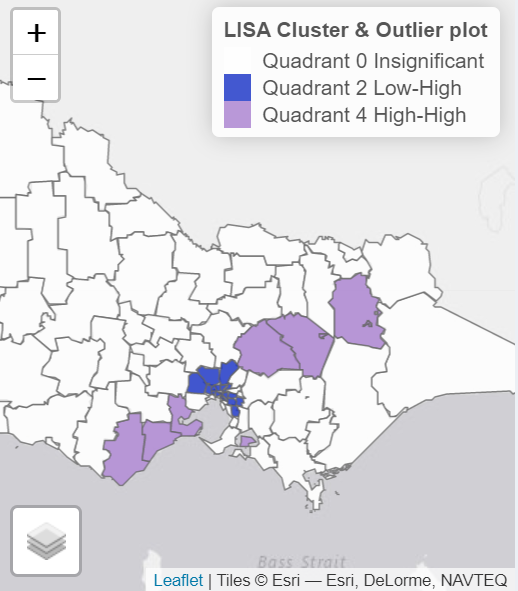
\includegraphics{images/geo3.png}

We observed that there is an area of Low-High outliers (dark blue) in
the north of the Melbourne Bay Area - these are outlier LGAs with lower
median price as compared to their surrounding neighbors, which have
higher median price for the Airbnb listings within. This is potentially
driven by the largely tourist hotspot in the Melbourne area that drives
Airbnb listing prices higher around the Low-High region we observed.

On the other hand, we also notice two distinct High-High clusters in
purple. These area reflects clusters or congregation of LGAs with higher
median Airbnb listing prices. The cluster on the southwestern end of the
bay area corresponds to the start point of the famous Great Ocean Road
and is hence not a surprise to have wide-spread area of high
accommodation prices. The cluster to the East, though, comprises of
mainly smaller and more remote tourist spots such as the Swifts Creek -
the fact that they are detected as a High-High cluster is a little
unexpected. However, once we shift to take a look at the raw median
price (see viz in Section 5.3), we notice that this is mainly due to the
fact that surrounding LGAs typically have lower median price (since it
is a remote area) - any minor hotspot that increases the median listing
price slightly (though statistically significant) in LGAs of close
proximity (each with one small attraction) would result in a
``High-High'' cluster. This is confirmed when we notice the raw median
price of this cluster is of lower price range (ligher pink) than those
in the Great Ocean Road area.

\hypertarget{sentiment-analysis-1}{%
\subsection{Sentiment Analysis}\label{sentiment-analysis-1}}

Sentiment analysis with this app consists of a word cloud and topic
modelling using Latent Dirichlet Allocation (LDA). For this
demonstration, the region of Victoria, Australia, is selected. The
review scores range of 91 to 100 is also selected.

\hypertarget{word-cloud-1}{%
\subsubsection{Word Cloud}\label{word-cloud-1}}

With the above filter selections, the word cloud created is shown below.

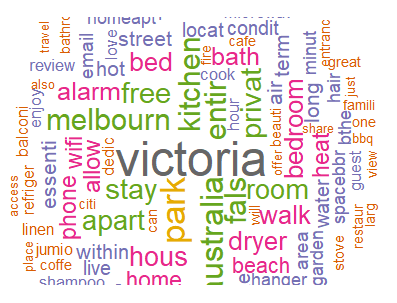
\includegraphics{images/wordcloud2.png} \emph{Figure 3: Word Cloud}

It is not unexpected that the word ``victoria'' is the most common word
in this word cloud, since the region in question here is Victoria. Some
other common words are ``kitchen,'' ``park,'' ``privat'' (private),
``bed,''bedroom``, and''walk".

This would suggest that these words are common in the descriptions that
hosts write about their listings, and these listings garner review score
ratings of 91 and above, which is the highest decile of review scores.
Thus for an Airbnb host who aims to obtain review score ratings within
that range, they should include these words into their descriptions. Of
course, the accommodation itself should actually offer these facilities
so as not to dissapoint the guest, which would expectedly lead to lower
rating scores.

\hypertarget{topic-modelling}{%
\subsubsection{Topic Modelling}\label{topic-modelling}}

Similar to the word cloud,the region of Victoria, Australia, is selected
with the review scores range of 91 to 100. The number of topics to be
identified is three, with the top ten words of each topic presented in
the visualisation.

With the above filter selections, the topic model is shown below.

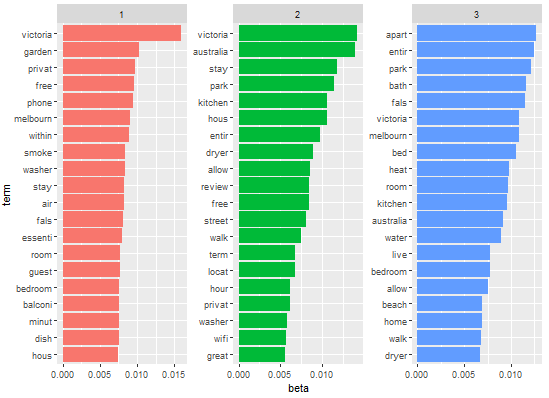
\includegraphics{images/topicmodel2.png} \emph{Figure 4: Topic Modelling
using LDA}

The bar beside the corresponding word represents the probability (beta)
of that word appearing in that particular topic. The longer the bar, the
higher the probability.

Based on the top words in each topic we can identify the following
topics:

\begin{itemize}
\item
  Topic 1: The word ``garden'' is very common in this topic (other than
  the word ``victoria'' which is the region in question). Along with
  ``garden,'' other words like ``phone,'' ``washer,'' ``essenti''
  (essentials), ``room,'' ``bedroom,'' ``balconi'' (balconies),
  ``minut'' (minutes) feature in the top 20 most common words in this
  cluster. This suggests that listing descriptions with these words tend
  to appeal to guests who stay in the accommodation more often, and
  enjoy facilities such as a garden, washer, balconies, etc. Such guests
  may be older persons who enjoy staying in the comforts of the house.
\item
  Topic 2: Words common to topic 2 are ``park,'' ``kitchen,'' ``dryer,''
  ``street,'' ``walk'' ``washer,'' ``wifi.'' These are some of the words
  in the list of top 20 most common words in this topic. This type of
  accommodation description may appeal more to younger guests who want
  Wi-Fi access in the accommodation, and also who might enjoy going
  outdoors to the park for a walk.
\item
  Topic 3: The common words in this cluster are ``park,'' ``bath,''
  ``bed,''heat``,''bedroom``,''beach``,''walk``,''dryer". These terms
  may appeal to those who are looking to visit the beach during their
  stay.
\end{itemize}

\hypertarget{discussion}{%
\section{Discussion}\label{discussion}}

\emph{(What has the audience learned from your work? What new insights
or practices has your system enabled? A full blown user study is not
expected, but informal observations of use that help evaluate your
system are encouraged.)}

The geospatial analysis allows audience to have a quick overview on the
geographical distribution of a variable of interest (say, median price)
across a selected level of detail (whole-of-Australia or individual
LGA). The LISA analysis further adds on to this overview to allow
identification of hotspots/coldspots (clusters of high/low value) and
outliers (LGAs with abnomally high/low median price vis-a-vis its
neighbors). User can form hypothesis about the spatial correlation
between different variable of interest (e.g.~price hotspots in Victoria
corresponds to rating hotspots), where further confirmatory analysis can
be conducted as an extension based on observations from this system. In
fact, with the clusters and outliers identified, users can conduct
deeper analysis on these areas using other tools available on this
system (e.g.~sentiment analysis, predictive analysis) to understand why
these patterns formed.

From the sentiment analysis, it was observed that most guests only gave
a review score if they has a positive experience staying at the
accommodation. As such, most of the review scores were in the range of
91 - 100. This caused a lack of data that could have highlighted what
words in a listing description might cause garner low review score
(claims of accommodation facilities that were not actually available,
for example), or what topics might receive the same (these topics might
reveal unpleasant sentiments for guests). However, it was still valuable
to know what terms and topics were common in listings that garnered high
review scores. Such insight would advise a potential host on what kind
of words or accommodation facilities would appeal more to guests. In
addition, different regions in Australia yield different results. For
example, the word cloud for Queensland yielded the terms ``Beach'' and
``park'' as the 2nd and 3rd most common terms, while the word cloud for
Queensland yielded only ``park.'' This indicates that Queensland
listings that garner high review scores are likely near a beach and made
that explicit in the listing description, whereas listings in Victoria
does not seem to have that, but still can highlight their proximity to
parks.

\hypertarget{future-work}{%
\section{Future Work}\label{future-work}}

\emph{(A description of how your system could be extended or refined.)}

Future versions of such an application could include other countries to
provide more comprehensive analysis of different regions and markets.
FOr example, Airbnb listings in South Africa may provide different
insight into what hosts provide and what guests want, compared to
Australia or other countries.

Other sentiment analysis techniques such as LSA could be included, to
provide the analyst with a more comprehensive suite of statistical
analysis tools with which to perform their analysis.

Deeper analysis could also be done on the profile of hosts as well as
guests, for example what type of hosts were more likely to have listings
that gained good reviews, or what type of guests were more likely to
match a certain type of listing and give good reviews.

On a whole-of-Australia scale, there are numerous LGAs with missing
data. In order support a more robust and holistic geospatial association
analysis, these information gaps will need to be plucked.

\hypertarget{references}{%
\section*{References}\label{references}}
\addcontentsline{toc}{section}{References}

\hypertarget{refs}{}
\begin{CSLReferences}{0}{0}
\leavevmode\hypertarget{ref-airbnb2020}{}%
\CSLLeftMargin{{[}1{]} }
\CSLRightInline{Airbnb 2020. 2020 Airbnb Update.}

\leavevmode\hypertarget{ref-abs}{}%
\CSLLeftMargin{{[}2{]} }
\CSLRightInline{Australian Bureau of Statistics 2020. Australian
Statistical Geography Standard (ASGS): Volume 3 - Non ABS Structure.}

\leavevmode\hypertarget{ref-brandeduc2019}{}%
\CSLLeftMargin{{[}3{]} }
\CSLRightInline{Brand Education 2019. Airbnb Inc.}

\leavevmode\hypertarget{ref-git2016}{}%
\CSLLeftMargin{{[}4{]} }
\CSLRightInline{Cvitanic, T. et al. 2016. LDA v. LSA: A Comparison of
Two Computational Text Analysis Tools for the Functional Categorization
of Patents.}

\leavevmode\hypertarget{ref-wikilda2021}{}%
\CSLLeftMargin{{[}5{]} }
\CSLRightInline{Latent Dirichlet allocation: 2021.
\emph{\url{https://en.wikipedia.org/wiki/Latent_Dirichlet_allocation}}.}

\leavevmode\hypertarget{ref-contiguityneigh}{}%
\CSLLeftMargin{{[}6{]} }
\CSLRightInline{Luc Anselin 2020. Contiguity-Based Spatial Weight.}

\leavevmode\hypertarget{ref-distanceneigh}{}%
\CSLLeftMargin{{[}7{]} }
\CSLRightInline{Luc Anselin 2018. Distance-Based Spatial Weight.}

\leavevmode\hypertarget{ref-cran2021}{}%
\CSLLeftMargin{{[}8{]} }
\CSLRightInline{The Comprehensive R Archive Network 2021. The
Comprehensive R Archive Network.}

\end{CSLReferences}
\setlength{\parindent}{0in}

\end{document}
